

\tikzset{every picture/.style={line width=0.75pt}} %set default line width to 0.75pt        

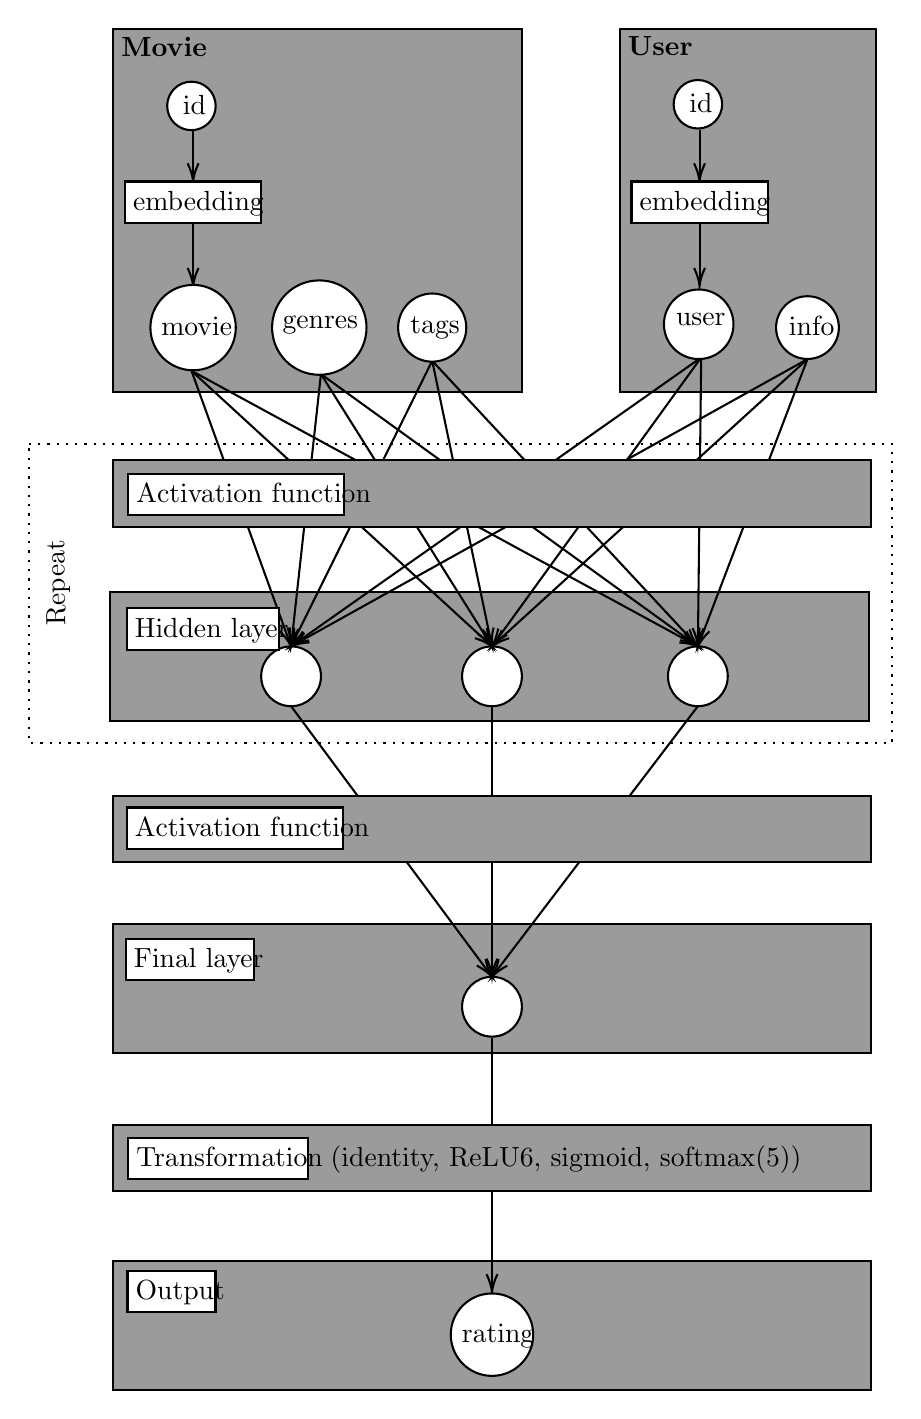
\begin{tikzpicture}[x=0.75pt,y=0.75pt,yscale=-1,xscale=1, scale=0.8]
%uncomment if require: \path (0,923); %set diagram left start at 0, and has height of 923

%Shape: Rectangle [id:dp2307314996446338] 
\draw  [fill={rgb, 255:red, 155; green, 155; blue, 155 }  ,fill opacity=1 ] (122,31) -- (368,31) -- (368,250) -- (122,250) -- cycle ;
%Straight Lines [id:da16141207798725943] 
\draw    (170,92) -- (170,121) ;
\draw [shift={(170,123)}, rotate = 270] [color={rgb, 255:red, 0; green, 0; blue, 0 }  ][line width=0.75]    (10.93,-3.29) .. controls (6.95,-1.4) and (3.31,-0.3) .. (0,0) .. controls (3.31,0.3) and (6.95,1.4) .. (10.93,3.29)   ;
%Straight Lines [id:da256251158457261] 
\draw    (170,148) -- (170,184) ;
\draw [shift={(170,186)}, rotate = 270] [color={rgb, 255:red, 0; green, 0; blue, 0 }  ][line width=0.75]    (10.93,-3.29) .. controls (6.95,-1.4) and (3.31,-0.3) .. (0,0) .. controls (3.31,0.3) and (6.95,1.4) .. (10.93,3.29)   ;
%Shape: Rectangle [id:dp4062601423389237] 
\draw  [fill={rgb, 255:red, 155; green, 155; blue, 155 }  ,fill opacity=1 ] (427,31) -- (581,31) -- (581,250) -- (427,250) -- cycle ;
%Straight Lines [id:da5944797488705584] 
\draw    (475,92) -- (475,121) ;
\draw [shift={(475,123)}, rotate = 270] [color={rgb, 255:red, 0; green, 0; blue, 0 }  ][line width=0.75]    (10.93,-3.29) .. controls (6.95,-1.4) and (3.31,-0.3) .. (0,0) .. controls (3.31,0.3) and (6.95,1.4) .. (10.93,3.29)   ;
%Straight Lines [id:da3036173249772247] 
\draw    (475,148) -- (475,184) ;
\draw [shift={(475,186)}, rotate = 270] [color={rgb, 255:red, 0; green, 0; blue, 0 }  ][line width=0.75]    (10.93,-3.29) .. controls (6.95,-1.4) and (3.31,-0.3) .. (0,0) .. controls (3.31,0.3) and (6.95,1.4) .. (10.93,3.29)   ;
%Shape: Rectangle [id:dp9997854452663028] 
\draw  [fill={rgb, 255:red, 155; green, 155; blue, 155 }  ,fill opacity=1 ] (120,370) -- (577,370) -- (577,448) -- (120,448) -- cycle ;
%Straight Lines [id:da5917985818254904] 
\draw    (169,237) -- (228.32,401.12) ;
\draw [shift={(229,403)}, rotate = 250.13] [color={rgb, 255:red, 0; green, 0; blue, 0 }  ][line width=0.75]    (10.93,-3.29) .. controls (6.95,-1.4) and (3.31,-0.3) .. (0,0) .. controls (3.31,0.3) and (6.95,1.4) .. (10.93,3.29)   ;
%Shape: Circle [id:dp6114587760100195] 
\draw  [fill={rgb, 255:red, 255; green, 255; blue, 255 }  ,fill opacity=1 ] (332,421) .. controls (332,411.06) and (340.06,403) .. (350,403) .. controls (359.94,403) and (368,411.06) .. (368,421) .. controls (368,430.94) and (359.94,439) .. (350,439) .. controls (340.06,439) and (332,430.94) .. (332,421) -- cycle ;
%Shape: Circle [id:dp553345531736126] 
\draw  [fill={rgb, 255:red, 255; green, 255; blue, 255 }  ,fill opacity=1 ] (456,421) .. controls (456,411.06) and (464.06,403) .. (474,403) .. controls (483.94,403) and (492,411.06) .. (492,421) .. controls (492,430.94) and (483.94,439) .. (474,439) .. controls (464.06,439) and (456,430.94) .. (456,421) -- cycle ;
%Shape: Circle [id:dp16008652747984975] 
\draw  [fill={rgb, 255:red, 255; green, 255; blue, 255 }  ,fill opacity=1 ] (211,421) .. controls (211,411.06) and (219.06,403) .. (229,403) .. controls (238.94,403) and (247,411.06) .. (247,421) .. controls (247,430.94) and (238.94,439) .. (229,439) .. controls (219.06,439) and (211,430.94) .. (211,421) -- cycle ;
%Straight Lines [id:da07936131606411578] 
\draw    (169,237) -- (472.24,402.04) ;
\draw [shift={(474,403)}, rotate = 208.56] [color={rgb, 255:red, 0; green, 0; blue, 0 }  ][line width=0.75]    (10.93,-3.29) .. controls (6.95,-1.4) and (3.31,-0.3) .. (0,0) .. controls (3.31,0.3) and (6.95,1.4) .. (10.93,3.29)   ;
%Straight Lines [id:da03140198678455175] 
\draw    (169,237) -- (348.53,401.65) ;
\draw [shift={(350,403)}, rotate = 222.52] [color={rgb, 255:red, 0; green, 0; blue, 0 }  ][line width=0.75]    (10.93,-3.29) .. controls (6.95,-1.4) and (3.31,-0.3) .. (0,0) .. controls (3.31,0.3) and (6.95,1.4) .. (10.93,3.29)   ;
%Straight Lines [id:da8972801381289985] 
\draw    (247,239) -- (229.22,401.01) ;
\draw [shift={(229,403)}, rotate = 276.26] [color={rgb, 255:red, 0; green, 0; blue, 0 }  ][line width=0.75]    (10.93,-3.29) .. controls (6.95,-1.4) and (3.31,-0.3) .. (0,0) .. controls (3.31,0.3) and (6.95,1.4) .. (10.93,3.29)   ;
%Straight Lines [id:da5048950093422406] 
\draw    (247,239) -- (472.38,401.83) ;
\draw [shift={(474,403)}, rotate = 215.85] [color={rgb, 255:red, 0; green, 0; blue, 0 }  ][line width=0.75]    (10.93,-3.29) .. controls (6.95,-1.4) and (3.31,-0.3) .. (0,0) .. controls (3.31,0.3) and (6.95,1.4) .. (10.93,3.29)   ;
%Straight Lines [id:da2676023756738023] 
\draw    (247,239) -- (348.94,401.31) ;
\draw [shift={(350,403)}, rotate = 237.87] [color={rgb, 255:red, 0; green, 0; blue, 0 }  ][line width=0.75]    (10.93,-3.29) .. controls (6.95,-1.4) and (3.31,-0.3) .. (0,0) .. controls (3.31,0.3) and (6.95,1.4) .. (10.93,3.29)   ;
%Straight Lines [id:da4547393022990093] 
\draw    (314,231) -- (229.89,401.21) ;
\draw [shift={(229,403)}, rotate = 296.3] [color={rgb, 255:red, 0; green, 0; blue, 0 }  ][line width=0.75]    (10.93,-3.29) .. controls (6.95,-1.4) and (3.31,-0.3) .. (0,0) .. controls (3.31,0.3) and (6.95,1.4) .. (10.93,3.29)   ;
%Straight Lines [id:da6479494477610002] 
\draw    (314,231) -- (472.64,401.54) ;
\draw [shift={(474,403)}, rotate = 227.07] [color={rgb, 255:red, 0; green, 0; blue, 0 }  ][line width=0.75]    (10.93,-3.29) .. controls (6.95,-1.4) and (3.31,-0.3) .. (0,0) .. controls (3.31,0.3) and (6.95,1.4) .. (10.93,3.29)   ;
%Straight Lines [id:da443095768705153] 
\draw    (314,231) -- (349.59,401.04) ;
\draw [shift={(350,403)}, rotate = 258.18] [color={rgb, 255:red, 0; green, 0; blue, 0 }  ][line width=0.75]    (10.93,-3.29) .. controls (6.95,-1.4) and (3.31,-0.3) .. (0,0) .. controls (3.31,0.3) and (6.95,1.4) .. (10.93,3.29)   ;
%Straight Lines [id:da35507587145535247] 
\draw    (476,229) -- (424.1,265.56) -- (230.64,401.85) ;
\draw [shift={(229,403)}, rotate = 324.84000000000003] [color={rgb, 255:red, 0; green, 0; blue, 0 }  ][line width=0.75]    (10.93,-3.29) .. controls (6.95,-1.4) and (3.31,-0.3) .. (0,0) .. controls (3.31,0.3) and (6.95,1.4) .. (10.93,3.29)   ;
%Straight Lines [id:da9486617458047818] 
\draw    (476,229) -- (474.02,401) ;
\draw [shift={(474,403)}, rotate = 270.65999999999997] [color={rgb, 255:red, 0; green, 0; blue, 0 }  ][line width=0.75]    (10.93,-3.29) .. controls (6.95,-1.4) and (3.31,-0.3) .. (0,0) .. controls (3.31,0.3) and (6.95,1.4) .. (10.93,3.29)   ;
%Straight Lines [id:da8058732839276246] 
\draw    (476,229) -- (351.17,401.38) ;
\draw [shift={(350,403)}, rotate = 305.90999999999997] [color={rgb, 255:red, 0; green, 0; blue, 0 }  ][line width=0.75]    (10.93,-3.29) .. controls (6.95,-1.4) and (3.31,-0.3) .. (0,0) .. controls (3.31,0.3) and (6.95,1.4) .. (10.93,3.29)   ;
%Straight Lines [id:da8260388432043336] 
\draw    (540,230) -- (230.75,402.03) ;
\draw [shift={(229,403)}, rotate = 330.90999999999997] [color={rgb, 255:red, 0; green, 0; blue, 0 }  ][line width=0.75]    (10.93,-3.29) .. controls (6.95,-1.4) and (3.31,-0.3) .. (0,0) .. controls (3.31,0.3) and (6.95,1.4) .. (10.93,3.29)   ;
%Straight Lines [id:da9400545257458622] 
\draw    (540,230) -- (474.71,401.13) ;
\draw [shift={(474,403)}, rotate = 290.88] [color={rgb, 255:red, 0; green, 0; blue, 0 }  ][line width=0.75]    (10.93,-3.29) .. controls (6.95,-1.4) and (3.31,-0.3) .. (0,0) .. controls (3.31,0.3) and (6.95,1.4) .. (10.93,3.29)   ;
%Straight Lines [id:da05542791968584537] 
\draw    (540,230) -- (351.48,401.65) ;
\draw [shift={(350,403)}, rotate = 317.68] [color={rgb, 255:red, 0; green, 0; blue, 0 }  ][line width=0.75]    (10.93,-3.29) .. controls (6.95,-1.4) and (3.31,-0.3) .. (0,0) .. controls (3.31,0.3) and (6.95,1.4) .. (10.93,3.29)   ;
%Shape: Rectangle [id:dp9672123809852601] 
\draw  [fill={rgb, 255:red, 155; green, 155; blue, 155 }  ,fill opacity=1 ] (121.5,291) -- (578.5,291) -- (578.5,331) -- (121.5,331) -- cycle ;
%Shape: Rectangle [id:dp27962627521584915] 
\draw  [dash pattern={on 0.84pt off 2.51pt}] (71,281) -- (591,281) -- (591,461) -- (71,461) -- cycle ;
%Shape: Rectangle [id:dp7643196245006507] 
\draw  [fill={rgb, 255:red, 155; green, 155; blue, 155 }  ,fill opacity=1 ] (121.5,570) -- (578.5,570) -- (578.5,648) -- (121.5,648) -- cycle ;
%Shape: Circle [id:dp2621970126778864] 
\draw  [fill={rgb, 255:red, 255; green, 255; blue, 255 }  ,fill opacity=1 ] (332,620) .. controls (332,610.06) and (340.06,602) .. (350,602) .. controls (359.94,602) and (368,610.06) .. (368,620) .. controls (368,629.94) and (359.94,638) .. (350,638) .. controls (340.06,638) and (332,629.94) .. (332,620) -- cycle ;
%Straight Lines [id:da7681063443100834] 
\draw    (229,439) -- (348.81,600.39) ;
\draw [shift={(350,602)}, rotate = 233.41] [color={rgb, 255:red, 0; green, 0; blue, 0 }  ][line width=0.75]    (10.93,-3.29) .. controls (6.95,-1.4) and (3.31,-0.3) .. (0,0) .. controls (3.31,0.3) and (6.95,1.4) .. (10.93,3.29)   ;
%Straight Lines [id:da5530075765034418] 
\draw    (350,439) -- (350,600) ;
\draw [shift={(350,602)}, rotate = 270] [color={rgb, 255:red, 0; green, 0; blue, 0 }  ][line width=0.75]    (10.93,-3.29) .. controls (6.95,-1.4) and (3.31,-0.3) .. (0,0) .. controls (3.31,0.3) and (6.95,1.4) .. (10.93,3.29)   ;
%Straight Lines [id:da8488306912122049] 
\draw    (474,439) -- (351.21,600.41) ;
\draw [shift={(350,602)}, rotate = 307.26] [color={rgb, 255:red, 0; green, 0; blue, 0 }  ][line width=0.75]    (10.93,-3.29) .. controls (6.95,-1.4) and (3.31,-0.3) .. (0,0) .. controls (3.31,0.3) and (6.95,1.4) .. (10.93,3.29)   ;
%Shape: Rectangle [id:dp9887981961930326] 
\draw  [fill={rgb, 255:red, 155; green, 155; blue, 155 }  ,fill opacity=1 ] (121.5,493) -- (578.5,493) -- (578.5,533) -- (121.5,533) -- cycle ;
%Shape: Rectangle [id:dp18515621761343992] 
\draw  [fill={rgb, 255:red, 155; green, 155; blue, 155 }  ,fill opacity=1 ] (121.5,773) -- (578.5,773) -- (578.5,851) -- (121.5,851) -- cycle ;
%Straight Lines [id:da2322651311514875] 
\draw    (350,639) -- (350,790) ;
\draw [shift={(350,792)}, rotate = 270] [color={rgb, 255:red, 0; green, 0; blue, 0 }  ][line width=0.75]    (10.93,-3.29) .. controls (6.95,-1.4) and (3.31,-0.3) .. (0,0) .. controls (3.31,0.3) and (6.95,1.4) .. (10.93,3.29)   ;
%Shape: Rectangle [id:dp7909457996411972] 
\draw  [fill={rgb, 255:red, 155; green, 155; blue, 155 }  ,fill opacity=1 ] (121.5,691) -- (578.5,691) -- (578.5,731) -- (121.5,731) -- cycle ;

% Text Node
\draw (125,34) node [anchor=north west][inner sep=0.75pt]   [align=left] {\textbf{Movie}};
% Text Node
\draw  [fill={rgb, 255:red, 255; green, 255; blue, 255 }  ,fill opacity=1 ]  (169, 77.5) circle [x radius= 14.6, y radius= 14.6]   ;
\draw (162,69) node [anchor=north west][inner sep=0.75pt]   [align=left] {id};
% Text Node
\draw  [fill={rgb, 255:red, 255; green, 255; blue, 255 }  ,fill opacity=1 ]  (246, 211) circle [x radius= 28.43, y radius= 28.43]   ;
\draw (222,202.5) node [anchor=north west][inner sep=0.75pt]   [align=left] {genres};
% Text Node
\draw  [fill={rgb, 255:red, 255; green, 255; blue, 255 }  ,fill opacity=1 ]  (314, 211) circle [x radius= 20.52, y radius= 20.52]   ;
\draw (299,202.5) node [anchor=north west][inner sep=0.75pt]   [align=left] {tags};
% Text Node
\draw  [fill={rgb, 255:red, 255; green, 255; blue, 255 }  ,fill opacity=1 ]  (129,123) -- (211,123) -- (211,148) -- (129,148) -- cycle  ;
\draw (132,127) node [anchor=north west][inner sep=0.75pt]   [align=left] {embedding};
% Text Node
\draw  [fill={rgb, 255:red, 255; green, 255; blue, 255 }  ,fill opacity=1 ]  (170, 211) circle [x radius= 25.71, y radius= 25.71]   ;
\draw (149,202.5) node [anchor=north west][inner sep=0.75pt]   [align=left] {movie};
% Text Node
\draw (430,34) node [anchor=north west][inner sep=0.75pt]   [align=left] {\textbf{User}};
% Text Node
\draw  [fill={rgb, 255:red, 255; green, 255; blue, 255 }  ,fill opacity=1 ]  (474, 76.5) circle [x radius= 14.6, y radius= 14.6]   ;
\draw (467,68) node [anchor=north west][inner sep=0.75pt]   [align=left] {id};
% Text Node
\draw  [fill={rgb, 255:red, 255; green, 255; blue, 255 }  ,fill opacity=1 ]  (540, 211) circle [x radius= 18.9, y radius= 18.9]   ;
\draw (527,202.5) node [anchor=north west][inner sep=0.75pt]   [align=left] {info};
% Text Node
\draw  [fill={rgb, 255:red, 255; green, 255; blue, 255 }  ,fill opacity=1 ]  (434,123) -- (516,123) -- (516,148) -- (434,148) -- cycle  ;
\draw (437,127) node [anchor=north west][inner sep=0.75pt]   [align=left] {embedding};
% Text Node
\draw  [fill={rgb, 255:red, 255; green, 255; blue, 255 }  ,fill opacity=1 ]  (474.5, 209) circle [x radius= 20.94, y radius= 20.94]   ;
\draw (459,200.5) node [anchor=north west][inner sep=0.75pt]   [align=left] {user};
% Text Node
\draw  [fill={rgb, 255:red, 255; green, 255; blue, 255 }  ,fill opacity=1 ]  (131,299) -- (261,299) -- (261,324) -- (131,324) -- cycle  ;
\draw (134,303) node [anchor=north west][inner sep=0.75pt]   [align=left] {Activation function};
% Text Node
\draw  [fill={rgb, 255:red, 255; green, 255; blue, 255 }  ,fill opacity=1 ]  (130,380) -- (222,380) -- (222,405) -- (130,405) -- cycle  ;
\draw (133,384) node [anchor=north west][inner sep=0.75pt]   [align=left] {Hidden layer};
% Text Node
\draw (79.86,392.62) node [anchor=north west][inner sep=0.75pt]  [rotate=-269.18] [align=left] {Repeat};
% Text Node
\draw  [fill={rgb, 255:red, 255; green, 255; blue, 255 }  ,fill opacity=1 ]  (130,500) -- (260,500) -- (260,525) -- (130,525) -- cycle  ;
\draw (133,504) node [anchor=north west][inner sep=0.75pt]   [align=left] {Activation function};
% Text Node
\draw  [fill={rgb, 255:red, 255; green, 255; blue, 255 }  ,fill opacity=1 ]  (129.5,579) -- (206.5,579) -- (206.5,604) -- (129.5,604) -- cycle  ;
\draw (132.5,583) node [anchor=north west][inner sep=0.75pt]   [align=left] {Final layer};
% Text Node
\draw  [fill={rgb, 255:red, 255; green, 255; blue, 255 }  ,fill opacity=1 ]  (131,699) -- (239,699) -- (239,724) -- (131,724) -- cycle  ;
\draw (134,703) node [anchor=north west][inner sep=0.75pt]   [align=left] {Transformation};
% Text Node
\draw  [fill={rgb, 255:red, 255; green, 255; blue, 255 }  ,fill opacity=1 ]  (130.5,779) -- (183.5,779) -- (183.5,804) -- (130.5,804) -- cycle  ;
\draw (133.5,783) node [anchor=north west][inner sep=0.75pt]   [align=left] {Output};
% Text Node
\draw  [fill={rgb, 255:red, 255; green, 255; blue, 255 }  ,fill opacity=1 ]  (350, 817.5) circle [x radius= 24.82, y radius= 24.82]   ;
\draw (330,809) node [anchor=north west][inner sep=0.75pt]   [align=left] {rating};
% Text Node
\draw (251,702) node [anchor=north west][inner sep=0.75pt]   [align=left] {(identity, ReLU6, sigmoid, softmax(5))};


\end{tikzpicture}
